\section{Anatomy of a CBIR System}\label{sec:anatomy}

The inner workings of most CBIR systems can best be examined by looking at the
processing pipeline each query has to go through. The coarse sequence of
computational steps is almost the same in all such systems (Figure
\ref{fig:cbir_coarse_structure}):

\begin{enumerate}
    \item Acquire the image.
    \item Extract the signature using a feature extraction algorithm.
    \item Compare the signature to a database containing the signatures of the
        images to search within.
    \item Rank the images by similarity using the comparison results.
\end{enumerate}

\begin{figure}[h]
    \centering
    \subfloat[Local features]{%
        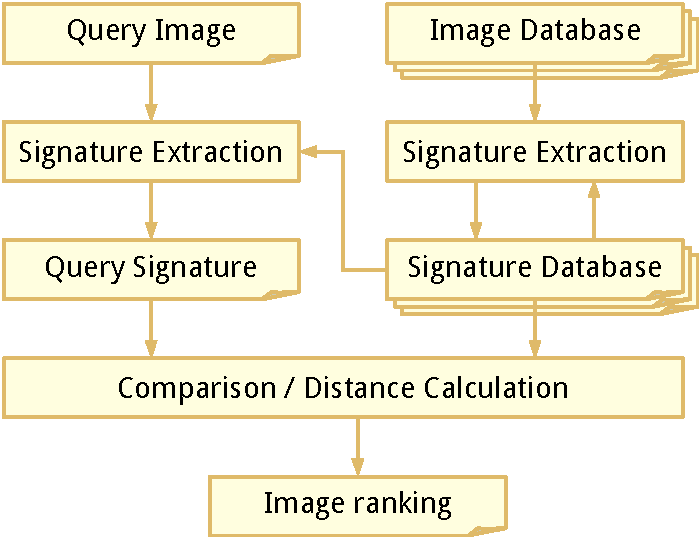
\includegraphics[width=0.45\textwidth]{cbir_anatomy_query_local_cropped}%
        \label{fig:cbir_coarse_structure_local}%
    }
    \quad
    \subfloat[Global features]{%
        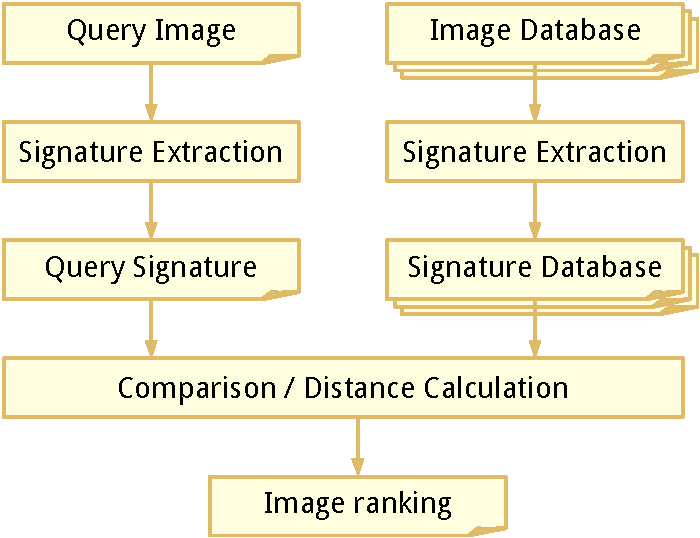
\includegraphics[width=0.45\textwidth]{cbir_anatomy_query_cropped}%
        \label{fig:cbir_coarse_structure_global}%
    }
    \caption[Coarse structure of a CBIR system]{
        The processing pipeline for CBIR using both local and global features
        is very similar. The main difference is in the signature extraction
        step, in which local features are selected, weighted and/or compressed
        depending on the results of the signature extraction of the other
        images in the database.
    }
    \label{fig:cbir_coarse_structure}
\end{figure}

\subsection{Image Acquisition}\label{sec:anatomy_image_acquisition}

The format in which the images are available to the system determines the
maximum amount of information available to subsequent analysis steps.

A significant part of the preprocessing usually done after acquisition depends
on the broadness of the image domain. The concept of the domain encompasses and
describes the variability of many possible image parameters like illumination
or composition and is therefore closely related to the sensory gap described
above. The narrower the image domain is, the more assumptions the system can
make about image from that domain. By their very nature, the domain of sketch
based image retrieval systems is usually very broad. It contains the sketches
create by the user to query the database as well as the images in the database
itself, which can be of a completely different nature, e.g.\ photos or
paintings.

Another factor usually is the accepted input format of the feature extraction
algorithm. Many algorithms like SIFT \autocite{lowe_object_1999} or SURF
\autocite{bay_speeded-up_2008} are defined for single-channel data, but some
have been specifically developed to operate on multi-channel images, like cSIFT
\autocite{abdel-hakim_csift:_2006} and \autocite{yang_robust_2008}.

\subsection{Signature Extraction}\label{sec:anatomy_signature_extraction}

The signature of an image is its representation in the following comparison
step. Therefore it should describe the image using its most discriminatory
features compared to all other images in the database. Due to the effects of
the \emph{sensory gap} discussed above, there is, at the moment, no definitive
way to determine the discriminatory power of features in general, even though
knowledge about the image domain can guide the descisions.  The signature
composition depends on both, the kind of features extracted from the image and
the way these features are encoded. 

Over the last two decades, a wide variety of feature descriptors have been
published, which mostly focus on specific types of features. Some techniques
use color histograms \autocite{utenpattanant_color_2006}, while others
\autocite{stricker_color_1996} \autocite{deng_efficient_2001}
\autocite{lee_spatial_2003} include spatial relations between colors in a
region.
Many descriptors attempt to capture texture characteristics, such as
\autocite{schaffalitzky_viewpoint_2001} and \autocite{manjunath_texture_1996}.
Rubner and Thomasi \autocite{rubner_texture-based_1999} combine Gabor filters
and the earth mover's distance and thereby bypass segmentation.
Another class of descriptors focuses on representing shapes using detection of
edges and salient points. Lowe \autocite{lowe_object_1999} developed the now
widely adopted SIFT descriptor, that employs clustering of salient points. More
recently, the SURF desciptor \autocite{bay_speeded-up_2008} uses Haar wavelets
to deliver comparable performance.
Several publications combine feature types to arrive at a more comprehensive
descriptor. Oliva and Torralba \autocite{oliva_modeling_2001} capture various
scene properties like "roughness" and "openness".

\subsubsection{Global Features}

Aside from the nature of the features captured by a descriptor, there are also
differences in the geometrical scope the features are derived from. Global
feature descriptors attempt to capture the structure of the whole scene or
describe the distribution of properties across the image like the binary Haar
color descriptor published in \autocite{utenpattanant_color_2006}. Some global
algorithms subdivide the image into regular segments and derive the localized
distribution of features for each division. \autocite{lazebnik_beyond_2006}
improves upon this concept by creating feature pyramids using iterative
subdivision for multiscale analysis. While the computational complexity of
those global approaches is usually quite low, they are especially susceptible
to problems like partial occlusion or reflections within the scene. The spatial
envelope descriptor \autocite{oliva_modeling_2001} combines a global
spectrogram with locally derived spectral information to produce an overall
image descriptor.

\subsubsection{Local Features}

In contrast to the global approach, many CBIR systems employ "bag-of-features"
descriptors, that represent the image as an unsorted collection of local
features extracted from small patches of the image. The unsorted nature of the
feature collection leads to loss of large-scale geometric structures that can
be counteracted by a suitable choice of the patch sizes. When the local feature
descriptors are invariant to rotation, scale or similar deformations, the
sensitivity to viewpoint variations or occlusions decreases. The prominent SIFT
descriptor \autocite{lowe_object_1999} achieves this by selecting the feature
locations such that they can be normalized with respect to scale, orientation
and limited 3D projections. The SURF descriptor by Bay et al
\autocite{bay_speeded-up_2008} gives similar results, but has reduces
computational requirements. The HOG descriptor \autocite{dalal_histograms_2005}
calculates histograms of gradient directions in a neighborhood.

\subsubsection{Dimensionality Reduction}

The signatures produced by local descriptors are often large sets of vector,
that are themselves of considerable size. For example, the SIFT descriptor
describes each image using about $1000$ local feature vectors of $160$ values
each. Such large numbers of vectors are expensive to store and compare, so one
of several data reduction methods is commonly used.

\paragraph{Principal Component Analysis}

The Principle Component Analysis (PCA) is a transformation, that computes the
orthogonal basis best suited to describe the variance of the data. An
$n$-dimensional data set is linearly mapped to a coordinate system, in which
the direction of the first axis $a_1$ is the direction with the largest
variance in the data. The following axes' $a_i$, $i \in 2, \dots, n$ directions
correspond to the orthogonal directions with the next-largest variances in
descending order. By choosing the $p$ largest component vectors and performing
an inverse transformation of the PCA-transformed data, a projection of the
original data in $p$ dimensions can be obtained. Due to the choice of the
vectors for the inverse transformation, the projection discards only the parts
of each observation that vary the least between all observations.

PCA has been applied to the face recognition problem using intensity images
(eigenfaces) \autocite{turk_face_1991}, wavelets (waveletfaces)
\autocite{feng_human_2000} and more recently curvelets (curveletfaces)
\autocite{mandal_face_2008}. In \autocite{ke_pca-sift:_2004} it was used to
improve the robustness of the SIFT \autocite{lowe_object_1999} descriptor. To
overcome the limited between-class discrimination of PCA, it has been combined
with Linear Discriminant Analysis (LDA), yielding even better results
\autocite{mandal_curvelet_2009}.

% k-means

\begin{figure}[h]
    \centering
        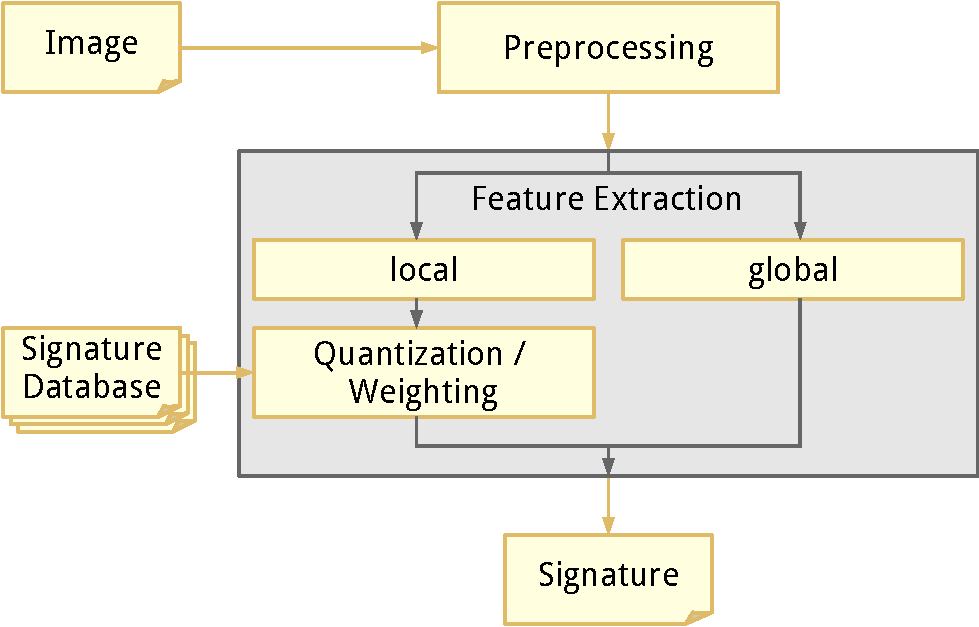
\includegraphics[width=0.8\textwidth]{cbir_anatomy_signature_extraction_cropped}
    \caption{Signature extraction in CBIR systems}
    \label{fig:cbir_signature_extraction}
\end{figure}

\subsection{Comparison and Ranking}\label{sec:anatomy_ranking}

TBD
